\chapter{Building Block View (Static View)}
\label{chapter{static_view}}

The following diagram shows the internal structure of RTA-SUM TCS:

%main diagram
\begin{figure}[h!]
	\centering
	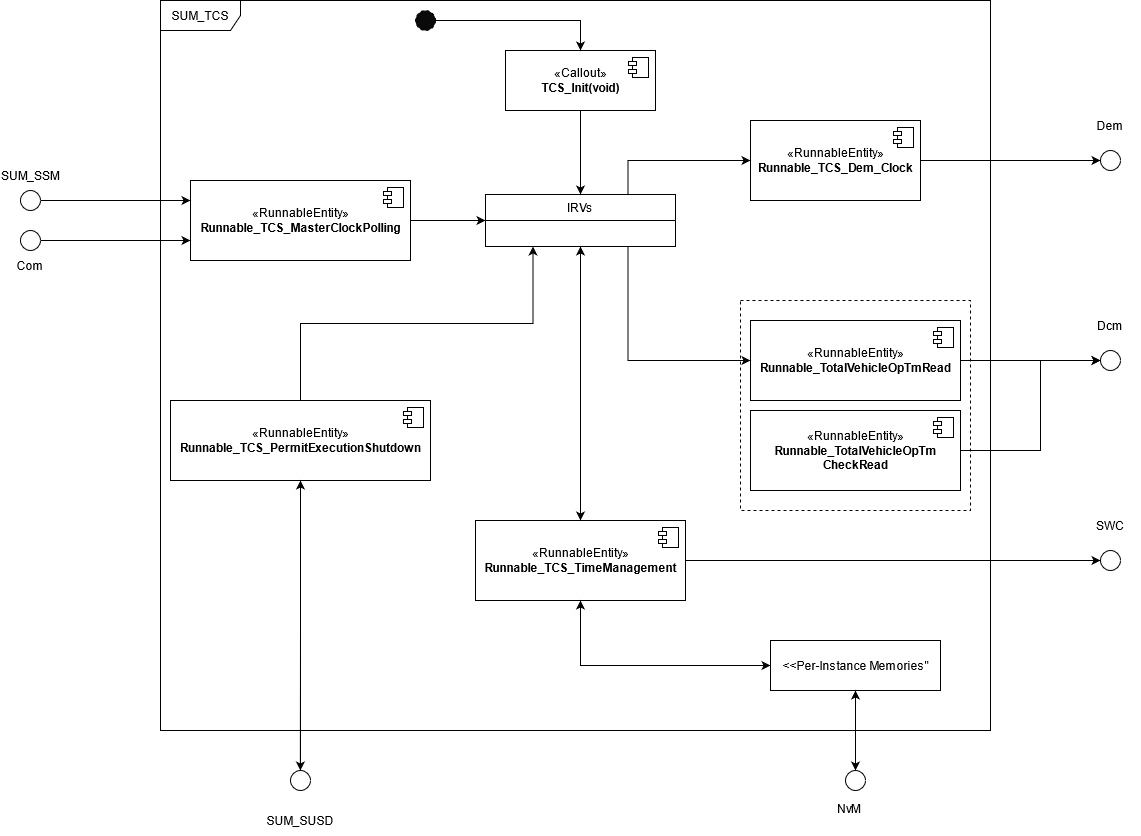
\includegraphics[scale=0.4]{images/TCSBlockDiagram.png}
	\caption{SUM\_TCS Block Diagram with Internal structure}
	\label{fig:block-diagram}
\end{figure}

The SUM\_TCS dependencies require that ECUs deploying the others SUMs:

\begin{itemize}
	\item SUM\_SSM: provider of signal availability for Time Synch Message;
	\item SUM\_SUSD: provider of Permit execution for requesting SUM\_TCS functionalities and BatteryVoltage_DisableNvmWrite condition and requester of shutdown permission information;
\end{itemize}

By means of the RTE, it also interacts with the following AUTOSAR BSW modules:

\begin{itemize}
	\item NvM;
	\item Dcm;
	\item Dem;
	\item COM;
\end{itemize}

And the SUM\_TCS can be able to send its local current computed time to any A-SWC that implements the appropriated port to receive it.
All blocks will be treated in deeper details in the following sections.

All variables must be designed in order to grant:

\begin{itemize}
	\item Consistency with respect to events, accesses and computations;
	\item Availability when they are accessed by specific Runnables in concurrency;
	\item Peristency of data during low power mode states;
\end{itemize}

SUM\_TCS protection mechanisms (as memory protections, and exclusive areas) are shown in the following to ensure the previous features.

\section{Port Interfaces}
\label{sec:PortInterfaces}

The following section reports the port-interfaces that are managed at the scope of SUM\_TCS utilization.
\\\\
If the port-interface name contain the keyword \textit{Configurable}, it means its multiplicity can be from 0 (not present) to N.
The port-interface name will contain a fix part (all that is not italic) and a dynamic part that will depend from configuration in arxml description.
\\\\
The port-interfaces scopes are specified in Interface description within the following table.

\textbf{CONSTRAINT}: ECU shall be able to support all ports types that are specified in the following table.

\textbf{LEGEND}:
\begin{itemize}
	\item \textit{S/R}: Sender-Receiver interface;
	\item \textit{C/S}: Client-Server interface;
	\item \textit{M/S}: Mode-Switch interface;
\end{itemize}

\RequirementTag{ADS_TCS}{001}
\input{generated/tables/portInterfaces}
{
	\Satisfies{SRS_TCS 003} \Satisfies{SRS_TCS 008} \Satisfies{SRS_TCS 009} \Satisfies{SRS_TCS 012} 
	\Satisfies{SRS_TCS 014} \Satisfies{SRS_TCS 015} \Satisfies{SRS_TCS 018} \Satisfies{SRS_TCS 019} 
	\Satisfies{SRS_TCS 023} \Satisfies{SRS_TCS 025} \Satisfies{SRS_TCS 027} \Satisfies{SRS_TCS 030} 
}

\section{Configuration}
\RequirementTag{ADS_TCS}{002}
\\
{\Satisfies{SRS_TCS 019}}
\\
SUM_TCS is a SWC within the context of AUTOSAR. It consists of static files and generated files.
SUM_TCS configuration is done the same way as for standard BSW modules: a parameter definition file is included with the module which allows users to configure the available parameters. 
Different configuration involves in different generated files for the same module. 
For default values of calibration parameters and others, SUM\_TCS is referring to the SDV-8002 or assumption on software requirements during development phase. 
Configuration parameters shall be pre-compile, i.e. the ECU behavior modification requires a reflash of the complete application software.

\subsection{Configuration Containers}
\label{subsec:ConfigurationContainers}

The following table contains information about the definition of configuration containers:

\input{generated/tables/containers_table}

Considering that module presents a single configuration container, no diagram is reported to represent the containers relationships.

\subsection{Configuration Parameters}

The following section reports all configuration parameters in scope to SUM\_TCS configuration. 
\\
Each configuration parameter shall involve in a pre-defined value or specific initialized data struct
that shall be used in reading mode for software component implementation.
\\
Pre-defined values that are involved from configuration parameters shall appear in \code{SUM\_TCS\_Cfg.h} and \code{SUM\_TCS\_Cfg.c}.

% 1
\input{generated/configurations/Conf_MasterClockPollingPeriodicity}\label{conf:MasterClockPollingPeriodicity}
\newline
{\textbf{Notes:} This value should be aligned to ECU gateway maximum latency for TimeSync message (GM defined to 100\code{ms})}
\newline

%2
\RequirementTag{ADS_TCS}{003}
\\
\input{generated/configurations/Conf_PermitExecutionMask}\label{conf:PermitExecutionMask}
\newline
{\textbf{Notes:} N/A}
\\
{\Satisfies{SRS_TCS 010}}
\newline

% 3
\input{generated/configurations/Conf_SumTCSGlobalTimePrecision}\label{conf:SumTCSGlobalTimePrecision}

\RequirementTag{ADS_TCS}{036}
\\
{\textbf{Notes:} Value shall be a multiple of \hyperref[conf:TimeManagementPeriodicity]{TimeManagementPeriodicity}. This constraints shall be validated during SUM\_TCS generation by OAW or other generation tool.\\
 let's use reasonable values. \textbf{No checking} on the feasibility of the value will be done a part from first point during configuration validation.}
 \\
{\Satisfies{SRS_TCS 017}}

% 4
\input{generated/configurations/Conf_TimeManagementPeriodicity}\label{conf:TimeManagementPeriodicity}
\newline
{\textbf{Notes:} The value of this configuration parameter shall be aligned to \hyperref[conf:MasterClockPollingPeriodicity]{MasterClockPollingPeriodicity} (as sub-multiple, or equals). A validation in SUM generation phase is required.
let's use feasible value. \textbf{No checking} on the feasibility of the value will be done a part from first point during configuration validation.}
\newline

\input{generated/configurations/Conf_TcsGenerateInitRunnable}\label{conf:TcsGenerateInitRunnable}
\newline
{\textbf{Notes:} N/A}
\newline

\input{generated/configurations/Conf_TcsInitFuncPeriodicity}\label{conf:TcsInitFuncPeriodicity}
\newline
{\textbf{Notes:} N/A}
\newline

The setting of values for configuration parameters define a particular \textit{Configuration}. Each \textit{Configuration} shall be able to satisfy some defined scenario with its related use case.

\subsection{Reference Parameters}
\label{sec:refparams}
\input{generated/references/DID_F129_TotalVehicleTimeValue_Reference}
\newline
{\textbf{Notes}: make reference to section \ref{sub:TotalVehicleTimeValue } for more information}

\input{generated/references/TcsDemTimestampRef}
\newline
{\textbf{Notes}: make reference to section \ref{sec:dtc-timestamp} for more information}

\subsection{Calibration Parameters}
No calibrations parameters are necessary at the scope of SUM\_TCS.

\section{Runnables}
\label{sec:Runnables}
\RequirementTag{ADS_TCS}{004}
\\
The runnables are used in order to manage the input and output interfaces for and from SUM\_TCS.
\\
Runnable execution shall be triggered by appropriated events according to managed interface type.
\\
According to SUM\_TCS interfaces, it requires 5 Runnables:
\\
{\Satisfies{SRS_TCS 001}}

\subsection{Runnable_TCS_MasterClockPolling}
This Runnable receives then computes the Master Clock Global Time message from COM in the application domain.
For more information refer to \ref{subsec:Runnable_TCS_MasterClockPolling}

\subsection{Runnable_TCS_TimeManagement}
This Runnable is responsible for updating the IRV counter and timers according to current status of SUM\_TCS operating mode.
For more information refer to \ref{subsec:Runnable_TCS_TimeManagement}

\subsection{Runnable_TCS_Dem_Clock}
This Runnable sends the current local time value to Dem for supporting the DTC Timestamp as extended data record;
For more information refer to \ref{subsec:Runnable_TCS_Dem_Clock}

\subsection{Runnable_TCS_PermitExecutionShutdown}
This Runnable is responsible for:
\begin{enumerate}
	\item Receive the permit execution value from SUM\_SUSD and updating the relative IRV;
	\item Manage the SUM\_TCS operating mode FSM;
	\item Request Memory services and check their execution;
	\item Provide the shutdown permission to SUM\_SUSD;
\end{enumerate}
For more information refer to \ref{subsec:Runnable_TCS_PermitExecutionShutdown}

\subsection{Runnable_RE_TCS_Init}
This Runnable is responsible for calling the \code{TCS_Init} when the configuration parameter \code{TcsGenerateInitRunnable} is set to TRUE.
For more information refer to \ref{subsec:RunnableTCSInit}

\subsection{Runnable_TotalVehicleTimeRead}
This runnable provides the callout function for supporting the \textbf{Reading} operation as UDS service 0x22 on DID 0xF129.
For more information refer to \ref{subsec:RunTotVehicleTimeRead}

\subsection{Runnable_TotalVehicleTimeCheckRead}
This runnable provides the callout function for supporting the \textbf{CheckRead} operation as UDS service 0x22 on DID 0xF129.
For more information refer to \ref{subsec:RunTotVehicleTimeCheckRead}

\section{Domain Data Structure and Utility blocks}

\subsection{Inter-runnable variables}
The following section describes the inter-runnable variables that are defined at SUM\_TCS scope:

\input{generated/inter_runnables_vars/list}

\todo{Create and use the following IRV as future TD activities}
{\textit{TCS_TimeManagementCounter}: This value is the main SUM\_TCS counter. Each ticks will match to a specific time that has been spent. It can be used as main counter for performing time divisions
to understand if a timer or counter shall be updated.}
\\
\\
{\textit{TCS_Permit_execution}: This value informs about the actual status for requesting the SUM\_TCS functionalities or not.}

\subsection{Per-Instance Memories}
SUM\_TCS implements Per-Instance memories as persistent memory mirror. Per-Instance memories that are implemented by SUM\_TCS are the following:

\begin{itemize}
	\item Initial value for local time computation (base value) that is loaded from Time synchronization message when it is received, \textbf{or}
	it is recovered from NvM;
	\input{generated/tables/SumTCSInitValue}
	\todo{Call it TCS_LocalTime_Value}
	\item Last value of TotalVehicleTimeValue  that is stored in NvM before each shutdown;
	\todo{Add a new Per-Instance Memory for TotalVehicleTimeValue }
\end{itemize}

\subsection{Utility functions}
\label{sec:utility-funcs}
This section designs the main scope of utility functions that implement specific services for SUM\_TCS in order to grant:

\begin{itemize}
	\item Reusability of Software units that implements common features;
	\item Low level of complexity in single unit;
\end{itemize}

The utility functions are C functions manually coded or model-based software designed and generated by coder.
\\
The utility functions belong to static part of the architecture, therefore they are dependent from current specification. If some static part in touch to utility functions will change,
the utility function will have to be changed in turn.
\\
\\
The main tasks in charge of Utility functions is to implement callbacks and callout for SUM\_TCS. The main services that are requested by SUM\_TCS are:

\begin{itemize}
	\item Read data from specific formats;
	\item Compute data according to request operations;
	\item Store results in appropriate data structure and containers;
	\item Perform checks and verification for implementing safety mechanisms;
\end{itemize}

\subsection{Data Identifiers Configuration}

\textbf{CONSTRAINT}: ECUs where SUM\_TCS is deployed must support UDS service 0x22.
\subsubsection{0xF129: TotalVehicleTimeValue }
\label{sub:TotalVehicleTimeValue }
SUM\_TCS shall compute, maintain and then provide to DID 0xF129 a running time counter that is called \textit{TotalVehicleTimeValue }, as response to UDS service 0x22;

\textbf{CONSTRAINT}: SUM\_TCS is implemented in ECU time slave, therefore service 0x2E cannot be available for DID 0x129.
\\
\\
SUM\_TCS shall provide TotalVehicleTimeValue  by appropriated interface to Dcm, and SUM\_TCS shall implement the callbacks for performing:

\begin{enumerate}
	\item Data read operation;
	\item CheckRead operation;
\end{enumerate}

\textbf{ASSUMPTION}: SUM\_TCS is implemented in order to have not any direct knowledge about status of PNs.
\\
It is assumed that SUM\_TCS will be activated from SUM\_SUSD whenever any PN is active in the system, \textbf{and} SUM\_TCS is asked to shutdown whenever no activity on PNs are detected for the system.

\begin{table}[h!]
	\centering
	\begin{tabular}{|c|l|}
		\hline
		\multicolumn{2}{|c|}{\cellcolor{ETASlightgray}\textbf{General Information}}\\
		\hline
		\cellcolor{ETASlightgray} \textit{Description} & Total time in which SUM\_TCS has detected activity on PNs.\\
		\hline
		\cellcolor{ETASlightgray} \textit{Scope} & local\\
		\hline
		\cellcolor{ETASlightgray} \textit{format} & 5-bytes (only 36-bits available) \\
		\hline
		\cellcolor{ETASlightgray} \textit{Sign} & unsigned \\
		\hline
		\cellcolor{ETASlightgray} \textit{Persistent Value} & The last computed before the module will go in shutdown\\
		\hline
		\cellcolor{ETASlightgray} \textit{Persistent Sorage} & NvM \\
		\hline
		\cellcolor{ETASlightgray} \textit{Default Endianess} & Little \\
		\hline
		\cellcolor{ETASlightgray} \textit{Range Values} & 0..6.871947673600E12\\
		\hline
		\cellcolor{ETASlightgray} \textit{Resolution} & 100\code{ms} for each counter tick \\
		\hline
	\end{tabular}
	\caption{TotalVehicleTimeValue }
	\label{tab:TotalVehicleTimeValue }
\end{table}

\RequirementTag{ADS_TCS}{005}
\\
TotalVehicleTimeValue  can be implemented as Per-Instance Memory and it can be updated each time that TCS_LocalTime_Clock reaches the number of ticks respective to (100\code{ms}/TimeManagementPeriodicity).
table \ref{tab:TotalVehicleTimeValue } defines main features of the type.
\\
{\Satisfies{SRS_TCS 025}}

\subsection{Diagnostic Trouble Codes Configuration}
\label{sec:dtc-timestamp}

\textbf{CONSTRAINT}: SUM\_TCS shall be implemented in an ECU that supports DTC setting.
\\
\\
\RequirementTag{ADS_TCS}{006}
\\
SUM\_TCS provides the timestamp value to Dem for DTC setting and reporting operations. Timestamp is considered in DTC operations as an extended data record.
\\
{\Satisfies{SRS_TCS 008}}
\\
\\
\textbf{CONSTRAINT}: SUM\_TCS is deployed in an ECU that supports UDS service 0x19.
\\
{
\label{paragraph:default-resolution}
Default time resolution for timestamp should be equal to the maximum delay of TimeSync message through to the ECU gateway, by default 100\code{ms}. Timestamp resolution can be configured as
configuration parameter
}
\\
\\
\RequirementTag{ADS_TCS}{007}
\\
Timestamp shall be:
\begin{itemize}
	\item Initialized with \textit{SumTCSInitValue}, until the reception of TimeSync message;
	\item Computed locally as incremental time counter that starts from a base;
	\item Computed with a time resolution equals to \textit{SumTCSGlobalTimePrecision};
	\item Saved in NvM (Persistent memory) when a shutdown request is going to be satisfied;
	\item Rebased (or re-synchronized) on:
	\begin{enumerate}
		\item Value in TimeSync message reception \textit{whenever it is received};
		\item Previous Timestamp value in NvM \textit{at the next startup after shutdown, if not 1};
	\end{enumerate}
\end{itemize}
{\Satisfies{SRS_TCS 007} \Satisfies{SRS_TCS 008}}

\textbf{ASSUMPTION}: The reading and writing operations on NvM may take some timing resources and then synchronization. This may have an impact on data integrity and in turn on safety aspects
of the Software component. So that the timestamp value shall be locally updated until a shutdown request does not occurr.

\begin{table}[h!]
	\centering
	\begin{tabular}{|c|l|}
		\hline
		\multicolumn{2}{|c|}{\cellcolor{ETASlightgray}\textbf{General Information}}\\
		\hline
		\cellcolor{ETASlightgray} \textit{Description} & computed time to be stored on NvM and provided to Dem as\\
		\cellcolor{ETASlightgray} & extended data record for DTC setting\\
		\hline
		\cellcolor{ETASlightgray} \textit{Scope} & local\\
		\hline
		\cellcolor{ETASlightgray} \textit{format} & 5-bytes \\
		\hline
		\cellcolor{ETASlightgray} \textit{Sign} & unsigned \\
		\hline
		\cellcolor{ETASlightgray} \textit{Persistent Value} & The last computed before the module  will go in shutdown\\
		\hline
		\cellcolor{ETASlightgray} \textit{Persistent Sorage} & NvM \\
		\hline
		\cellcolor{ETASlightgray} \textit{Default Endianess} & Little \\
		\hline
		\cellcolor{ETASlightgray} \textit{Range Values} & 0..1.099511627775E12\\
		\hline
		\cellcolor{ETASlightgray} \textit{Resolution} & \hyperref[conf:SumTCSGlobalTimePrecision]{SumTCSGlobalTimePrecision} \\
		\hline
	\end{tabular}
	\caption{Timestamp}
	\label{tab:timestamp}
\end{table}

\RequirementTag{ADS_TCS}{008}
\\
\textbf{NOTE}: Timestamp can be implemented as Per-Instance Memory and it can be updated each time that TCS_LocalTime_Clock reaches the number of ticks respective to (SUMTCSGlocalPrecisionTime/TimeManagementPeriodicity).
table \ref{tab:timestamp} defines main features of the type
\\
{\Satisfies{SRS_TCS 022}}


\subsection{Counters and Timers}

\subsubsection{TCS_TimeManagementCounter}
\label{sub:TimeManagementCounter}

The SUM\_TCS defines \textbf{counter} \textit{TCS_TimeManagementCounter} to count the number of execution times of the Runnable \hyperref[]{Runnable_TCS_TimeManagement} when SUM\_TCS is in active mode.
. The counter features are specified in table \ref{tab:TimeManagementCounter}.
 \begin{table}[h!]
	 \centering
	 \begin{tabular}{|c|l|}
		 \hline
		 \multicolumn{2}{|c|}{\cellcolor{ETASlightgray} \textbf{TCS_TimeManagementCounter}}\\
		 \hline
		 \cellcolor{ETASlightgray}\textit{Data size} & \code{4-Bytes}\\
		 \hline 
		 \cellcolor{ETASlightgray} \textit{Initial Value} & 0 \\
		 \hline
		 \cellcolor{ETASlightgray} \textit{Range} & 0..4294967295 \\
		 \hline
		 \cellcolor{ETASlightgray} \textit{Time resolution} & \hyperref[conf:TimeManagementPeriodicity]{TimeManagementPeriodicity}. \\
		 \hline
		 \cellcolor{ETASlightgray} \textit{Reset} & Initialization \\
		 \hline
		 \cellcolor{ETASlightgray} \textit{Enable} & module execution allowed \\
		 \hline
	 \end{tabular}
	 \caption{TimeManagementCounter general (High Level) design}
	 \label{tab:TimeManagementCounter}
 \end{table}